%Notes by Harsh Mistry 
%Econ 301
%Based on Template From  https://www.cs.cmu.edu/~ggordon/10725-F12/template.tex

\documentclass[twoside]{article}
\setlength{\oddsidemargin}{0.25 in}
\setlength{\evensidemargin}{-0.25 in}
\setlength{\topmargin}{-0.6 in}
\setlength{\textwidth}{6.5 in}
\setlength{\textheight}{8.5 in}
\setlength{\headsep}{0.75 in}
\setlength{\parindent}{0 in}
\setlength{\parskip}{0.1 in}
\usepackage{amsmath,amsfonts,graphicx, color}
\newcounter{lecnum}
\renewcommand{\thepage}{\thelecnum-\arabic{page}}
\renewcommand{\thesection}{\thelecnum.\arabic{section}}
\renewcommand{\theequation}{\thelecnum.\arabic{equation}}
\renewcommand{\thefigure}{\thelecnum.\arabic{figure}}
\renewcommand{\thetable}{\thelecnum.\arabic{table}}
\newcommand{\lecture}[4]{
   \pagestyle{myheadings}
   \thispagestyle{plain}
   \newpage
   \setcounter{lecnum}{#1}
   \setcounter{page}{1}
   
   
%Info Box 
   \begin{center}
   \framebox{
      \vbox{\vspace{2mm}
    \hbox to 6.28in { {\bf Econ 301 - Microeconomic Theory 2
	\hfill Winter 2018} }
       \vspace{4mm}
       \hbox to 6.28in { {\Large \hfill Lecture #1: #2  \hfill} }
       \vspace{2mm}
       \hbox to 6.28in { {\it Lecturer: #3 \hfill Notes By: #4} }
      \vspace{2mm}}
   }
   \end{center}
   
   \markboth{Lecture #1: #2}{Lecture #1: #2}



 
}

\renewcommand{\cite}[1]{[#1]}
\def\beginrefs{\begin{list}%
        {[\arabic{equation}]}{\usecounter{equation}
         \setlength{\leftmargin}{2.0truecm}\setlength{\labelsep}{0.4truecm}%
         \setlength{\labelwidth}{1.6truecm}}}
\def\endrefs{\end{list}}
\def\bibentry#1{\item[\hbox{[#1]}]}

\newcommand{\fig}[3]{
			\vspace{#2}
			\begin{center}
			Figure \thelecnum.#1:~#3
			\end{center}
	}
	
	\graphicspath{ {images/} }

\newtheorem{theorem}{Theorem}[lecnum]
\newtheorem{lemma}[theorem]{Lemma}
\newtheorem{ex}[theorem]{Example}
\newtheorem{proposition}[theorem]{Proposition}
\newtheorem{claim}[theorem]{Claim}
\newtheorem{corollary}[theorem]{Corollary}
\newtheorem{definition}[theorem]{Definition}
\newenvironment{proof}{{\bf Proof:}}{\hfill\rule{2mm}{2mm}}
\newcommand\E{\mathbb{E}}


%Start of Document 
\begin{document}

\lecture{13}{February 26, 2018}{Jean Guillaume Forand}{Harsh Mistry}

\section{Welfare Continued}
\begin{center}
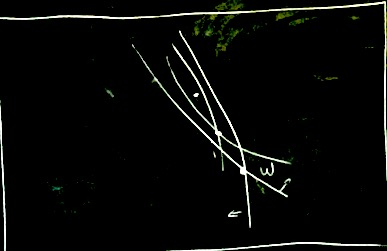
\includegraphics[scale=0.4]{21}
\end{center}
 \begin{definition}
 Allocations \(x^A\) and \(x^B\) \underline{Pareto dominante} allocations \(y^A\) and \(y^B\) if 
 \[u^J(x^J_1, x^J_2) \geq u^J(y^J_1, y^J_1) \text{ for all } J = 1, 2, \]
 with (at least) one inequality strict.
 \end{definition}

\begin{definition} \underline{Pareto-efficient} allocations \(x^A\) and \(x^B\) are not Pareto-dominated by any feasible allocations \(y^A\)and \(y^B\)
\end{definition}

\underline{Result} : Allocations consistent with bargaining between consumers are Pareto efficient allocations \(x^A\) and \(x^B\) such that \(u^J(x^J_1, x_2^J) \geq u^J(\omega^J_1, \omega^J_2)\) for all \(J = 1, 2\) \\

Pareto efficiency is fundamental normative criterion in economic. Basically, its not a strong argument, but its an criteria that can support your statement. 

\begin{itemize}
\item As a value judgement, Pareto is weak. Pareto-dominated allocations can be ruled out by unanimous votes
\item Pareto-efficient allocations are often unsatisfactory relative to additional normative criteria : (e.g no notion of fairness)
\item To find Pareto-efficient allocations :
\begin{itemize}
\item Start with allocations \(y^A\) and \(y^B\)
\item Find optimal allocations \(x^A\) and  \(x^B\) for consumer A such that consumer B is indifferent between \(x^B\) and \(y^B\)
\begin{center}
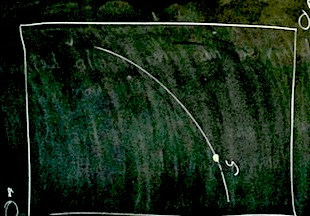
\includegraphics[scale=0.4]{22}
\end{center}
\item i.e. solution to UMP with equality constraint
\[ \max_{\{0 \leq x_i^A \leq \omega^A_i + \omega^B_i\}_{i=1,2}} u^A(x_1^A, x_2^A) \text{ s.t. } u^B(\omega_1^A + \omega_1^B - x_1^A, \omega_2^A + \omega^B_2 - x_2^B) = u^B(y_1^B, y_2^B)   \]
\item Lagrangian
\[L(x_1^A, x_2^A, \lambda) = u^A(x_1^A, x_2^A) + \lambda [u^B(y^B, y_2^B) - u^B(\omega_1^A - \omega_1^B - x_1^A , \omega_2^A + \omega_2^B - x_2^A)]\]
\item At an interior solution, we have the FOC
\[\frac{dL}{dx_i^A} (x_1^{A*}, x_2^{A*}, \lambda) =  \frac{d}{dx_i^A} u^A(x_1^A, x_2^A) + \lambda \frac{d}{dx_i^A} u^B(\omega_1^A - \omega_1^B - x_1^A , \omega_2^A + \omega_2^B - x_2^A)  = 0 \hspace{0.2cm} (Li), i =1, 2\]
\[\frac{dL}{d \lambda} (x_1^{A*}, x_2^{A*}, \lambda) =  0 \hspace{0.2cm} (L\lambda)\]
\item Let \(x_i^B = \omega^A_i + \omega_i^B - x_i^{A*}\)
\item Using (L1) - (L2) : 
\[\frac{\frac{d}{dx_1^{A}} u^A(x_1^A, x_2^A)}{\frac{d}{dx_2^A} u^A(x_1^A, x_2^A)} = \frac{\frac{d}{dx_1^B} u^B(x_1^B, x_2^B)}{\frac{d}{dx_2^B} u^B(x_1^B, x_2^B}\]
\item Result : If both consumers' preferences are monotone and convex, then the solutions to FOC are Pareto-efficient allocations. 
\begin{center}
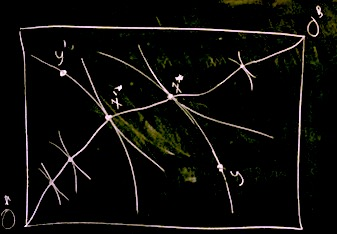
\includegraphics[scale=0.4]{23}
\end{center}
\item Allocations \(y^A\) and \(y^B\) are arbitrary, can find more Pareto-efficient allocations by considering different initial allocations 
\end{itemize}
\end{itemize}

\begin{definition}
The set of all Pareto-efficient allocations is the \underline{Pareto Set}, or \underline{contract curve}
\end{definition}
\newpage
\begin{ex} \(\omega^A = (1, 1), \omega^B = (1, 2), \omega^A(x^A_1, x^A_2) = x_1^{A \frac{1}{2}} x_2^{A \frac{1}{2}}, u^B(x_1^B, x_2^B) = x_1^{B \frac{1}{2}} x_2^{B \frac{1}{2}} \)
\begin{itemize}
\item Given allocations \(x^A\) and \(x^B\)
\[\frac{\frac{d}{dx_1^{A}} u^A(x_1^A, x_2^A)}{\frac{d}{dx_2^A} u^A(x_1^A, x_2^A)} = \frac{\frac{1}{2} \left(\frac{x_2^A}{x_1^A}\right)^\frac{1}{2}}{\frac{1}{2} \left(\frac{x_1^A}{x_2^A}\right)^\frac{1}{2}} = \frac{x_2^A}{x_1^A}\]
\[ \frac{\frac{d}{dx_1^B} u^B(x_1^B, x_2^B)}{\frac{d}{dx_2^B} u^B(x_1^B, x_2^B} = \frac{1}{3} \frac{x_2^B}{x_1^B}\]
\item Both consumers preferences are monotone and convex, so the Pareto set consists of all solutions to 
\[\frac{\frac{d}{dx_1^{A}} u^A(x_1^A, x_2^A)}{\frac{d}{dx_2^A} u^A(x_1^A, x_2^A)} = \frac{\frac{d}{dx_1^B} u^B(2-x_1^A, 2-x)2^A)}{\frac{d}{dx_2^B} u^B(2-x_1^A, 2-x)2^A)}\]
Or 
\[\frac{x_2^A}{x_1^A} = \frac{1}{3} \frac{3-x_2^A}{2-x_1^A}\]
\[x_2^A = \frac{3x_1^A}{2[3-x_1^A]}\]
\begin{center}
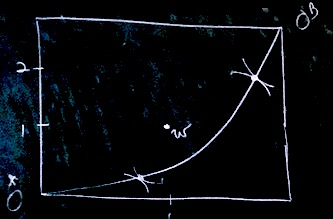
\includegraphics[scale=0.5]{24}
\end{center}
\end{itemize}
\end{ex} 

\end{document}





